\chapter{Introduction and Theory Overview} \label{Introduction and Theory Overview}

\section{Introduction}

\section{Theory}
%http://dx.doi.org/10.1016/j.physletb.2012.08.021
%http://www.sciencedirect.com/science/article/pii/S037026931200857X

The discovery of the boson whose mass around 125 GeV and with properties close to Higgs mechanism in the Standard model has incited the search under Higgs potential including Higgs self-coupling. Especially, it is a worth explored channel to finding new physic beyond Standard model. 
Targeting heavy resonance, the model Wraped Extra Dimension is considered. 

\subsection{Wraped Extra Dimension} 

\subsection{Motivation} 
%https://arxiv.org/pdf/1512.04357.pdf
There are models predicting heavy resonances decaying into VV.
%https://arxiv.org/abs/1506.00962
%https://arxiv.org/abs/1503.04677
%https://arxiv.org/abs/1409.6190
%https://arxiv.org/abs/1405.1994
Several researches on these channels are performed in both CMS and ATLAS.
There are also the combinations of these analyses.
%https://arxiv.org/abs/1405.3447
%https://arxiv.org/abs/1512.05099
The combination from ATLAS excludes the resonance of Bulk Graviton from below 810 GeV, and despit the combination from CMS fails to exclude any mass spectum of Bulk Graviton given a less sensitive model, it sets the upper limit of 10 fb of cross section of Bulk Graviton through $M_X$ from 600 to 2500 GeV.
%https://arxiv.org/pdf/1503.04114.pdf
%https://arxiv.org/pdf/1506.00285.pdf
Besides, searches for Bulk Graviton decaying into HH in four b-flavored quarks final state have been perfromed by CMS and ATLAS at $\sqrt{s}$ = 8 TeV. They exlude the mass region below 830 and 720 GeV respectively. The intermediate region of the mass of heavy resonances ( $M_X \thickapprox$ 2 TeV ) is left interesting to be explored.
 



%
%\begin{figure}[t]
%  \centering
%  \begin{tabular}{cc}
%    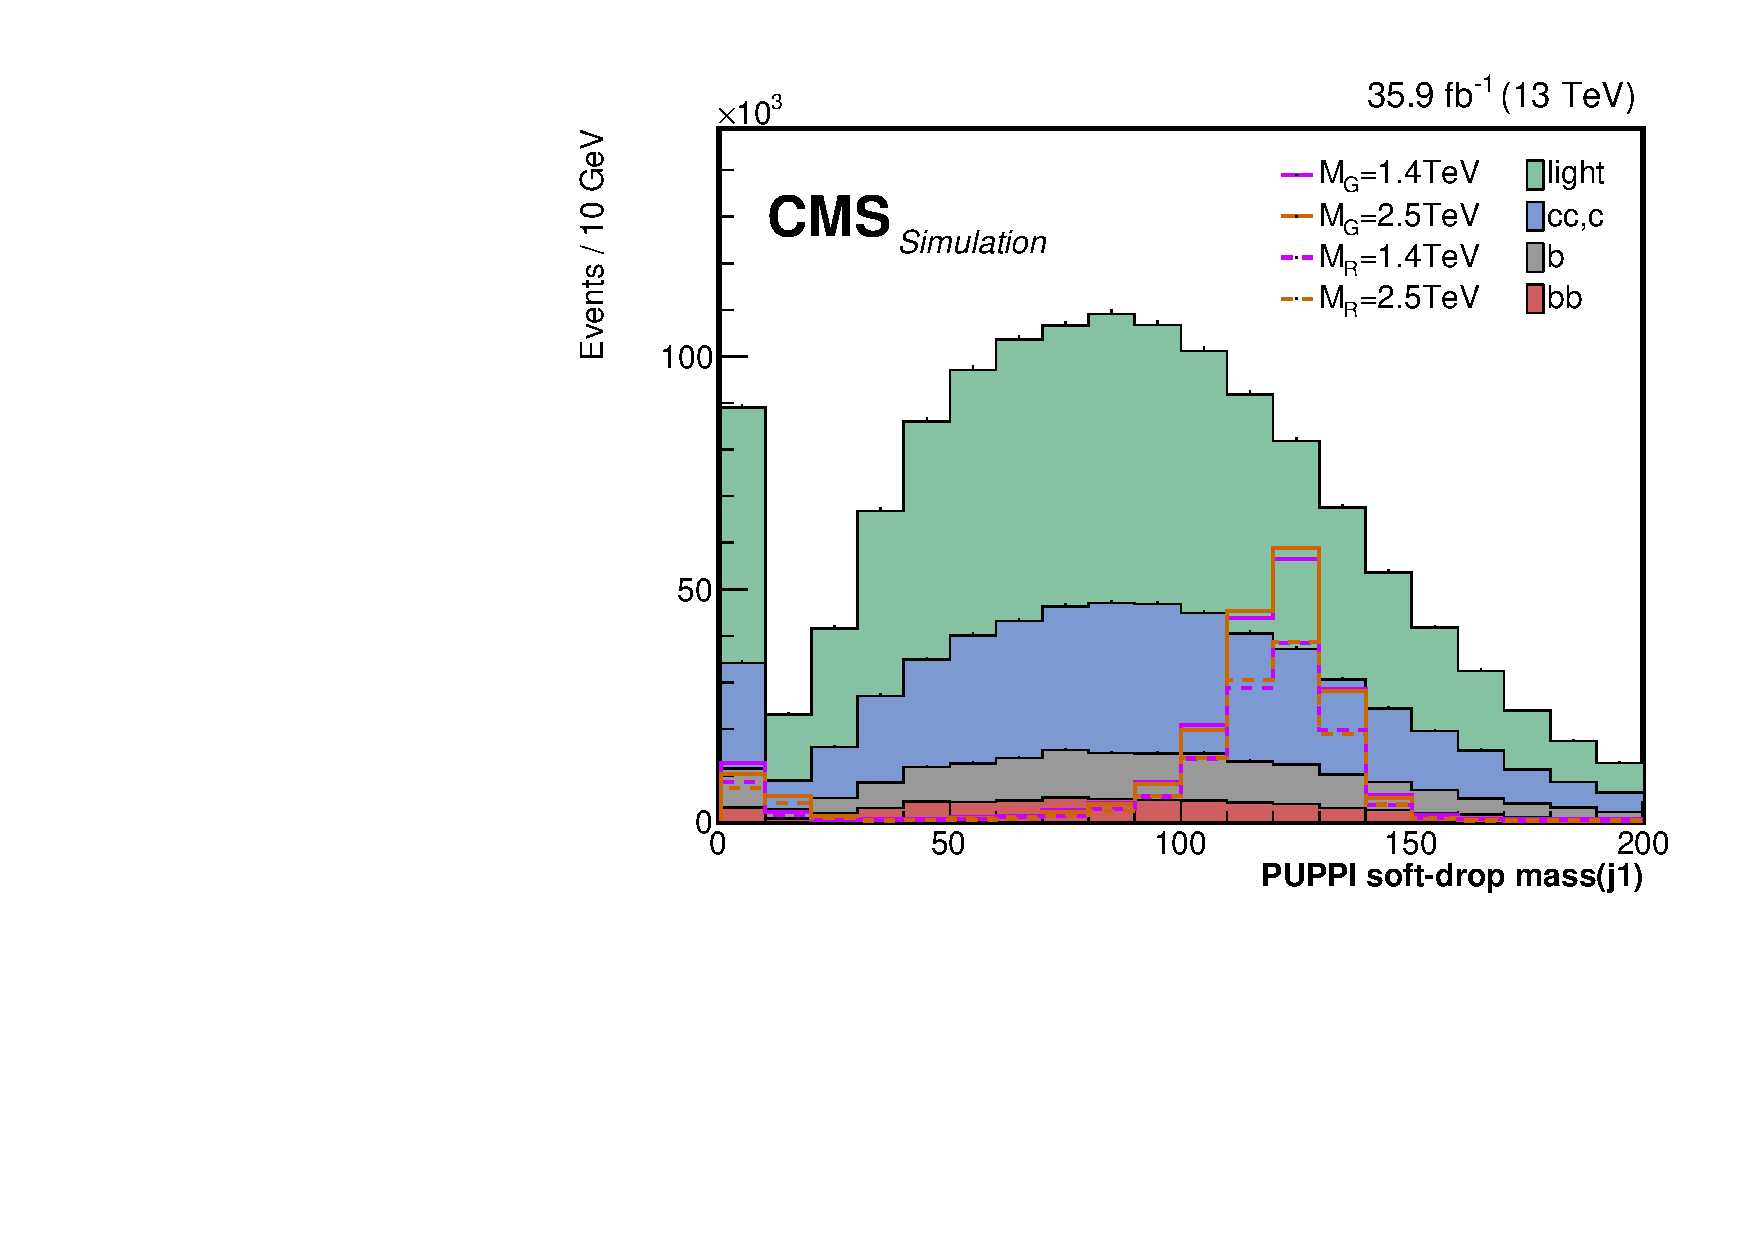
\includegraphics[width=0.5\textwidth]{Figures/MC_N1/puppiSDMassThea_j0.pdf} &
%    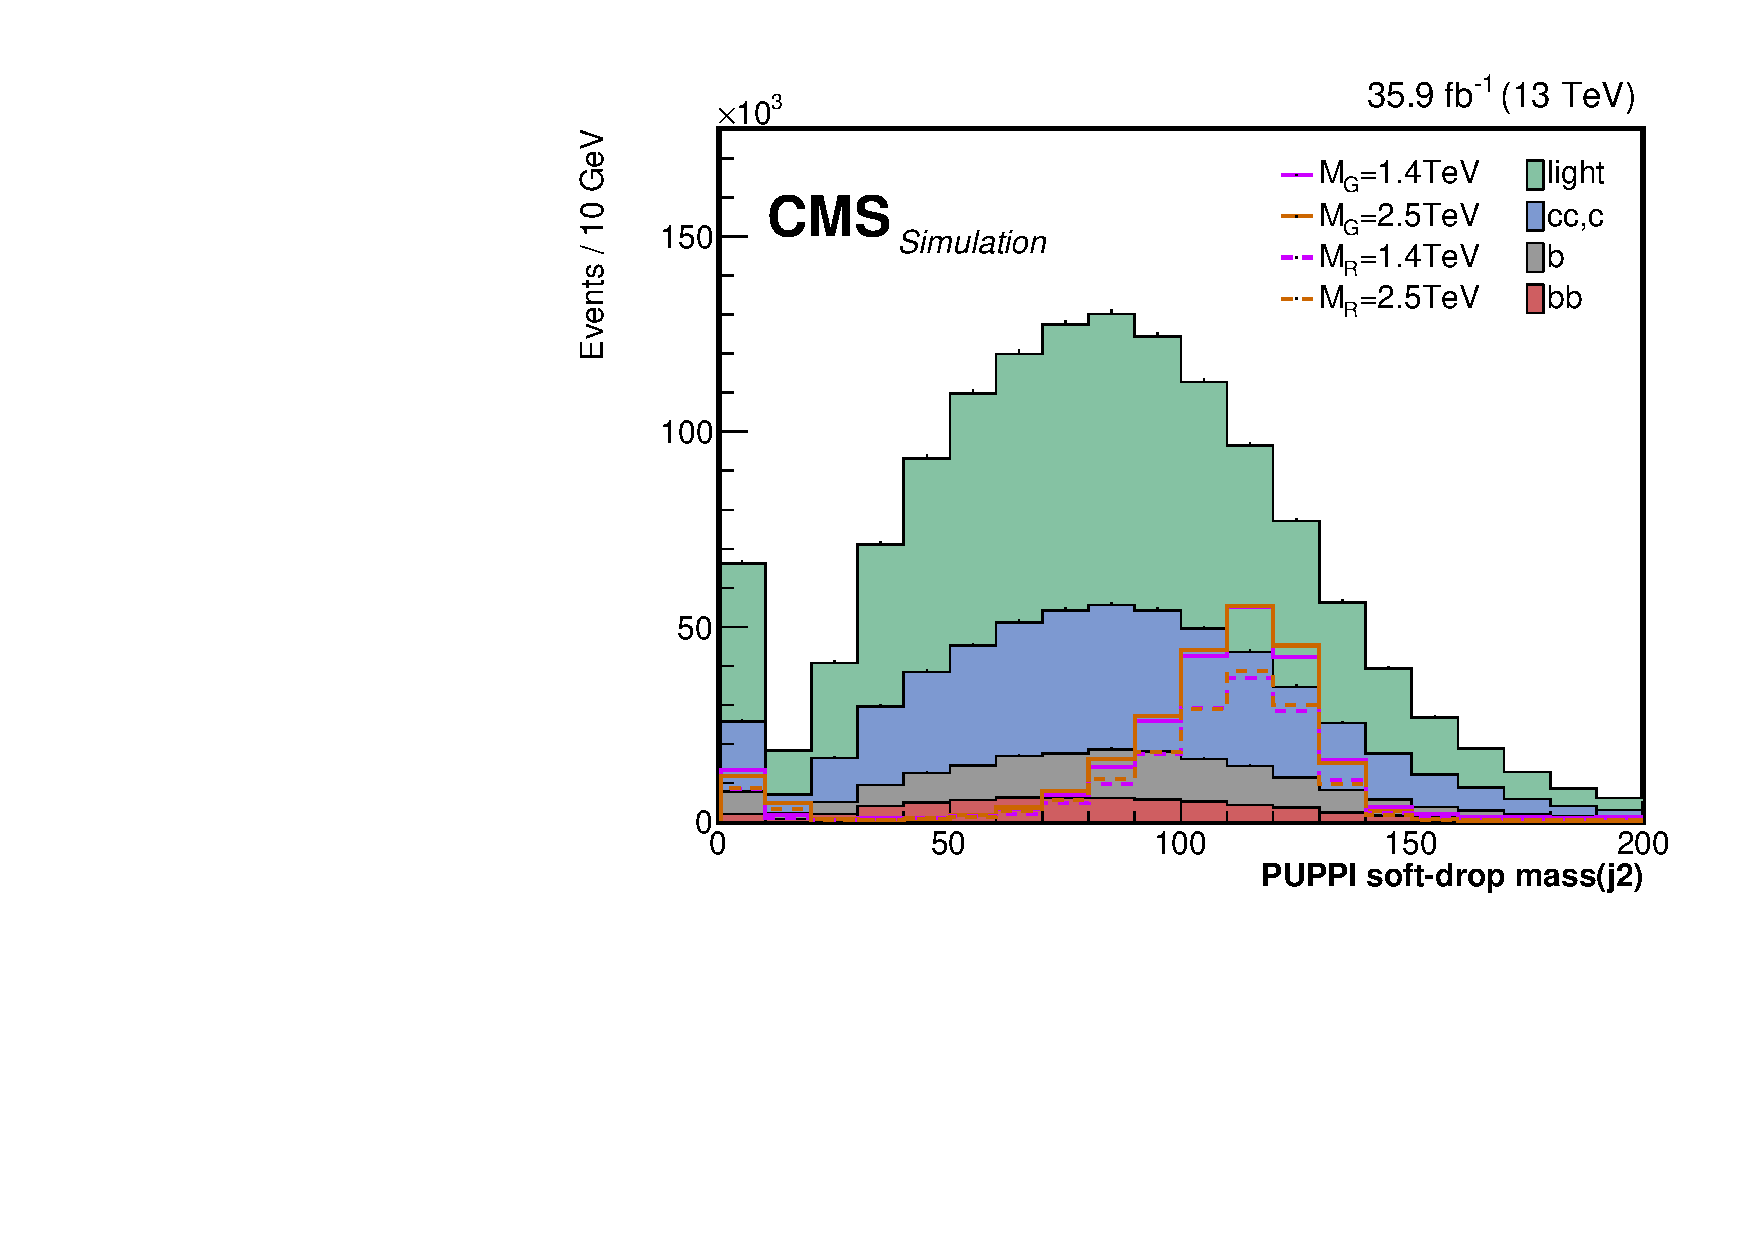
\includegraphics[width=0.5\textwidth]{Figures/MC_N1/puppiSDMassThea_j1.pdf} \\
%     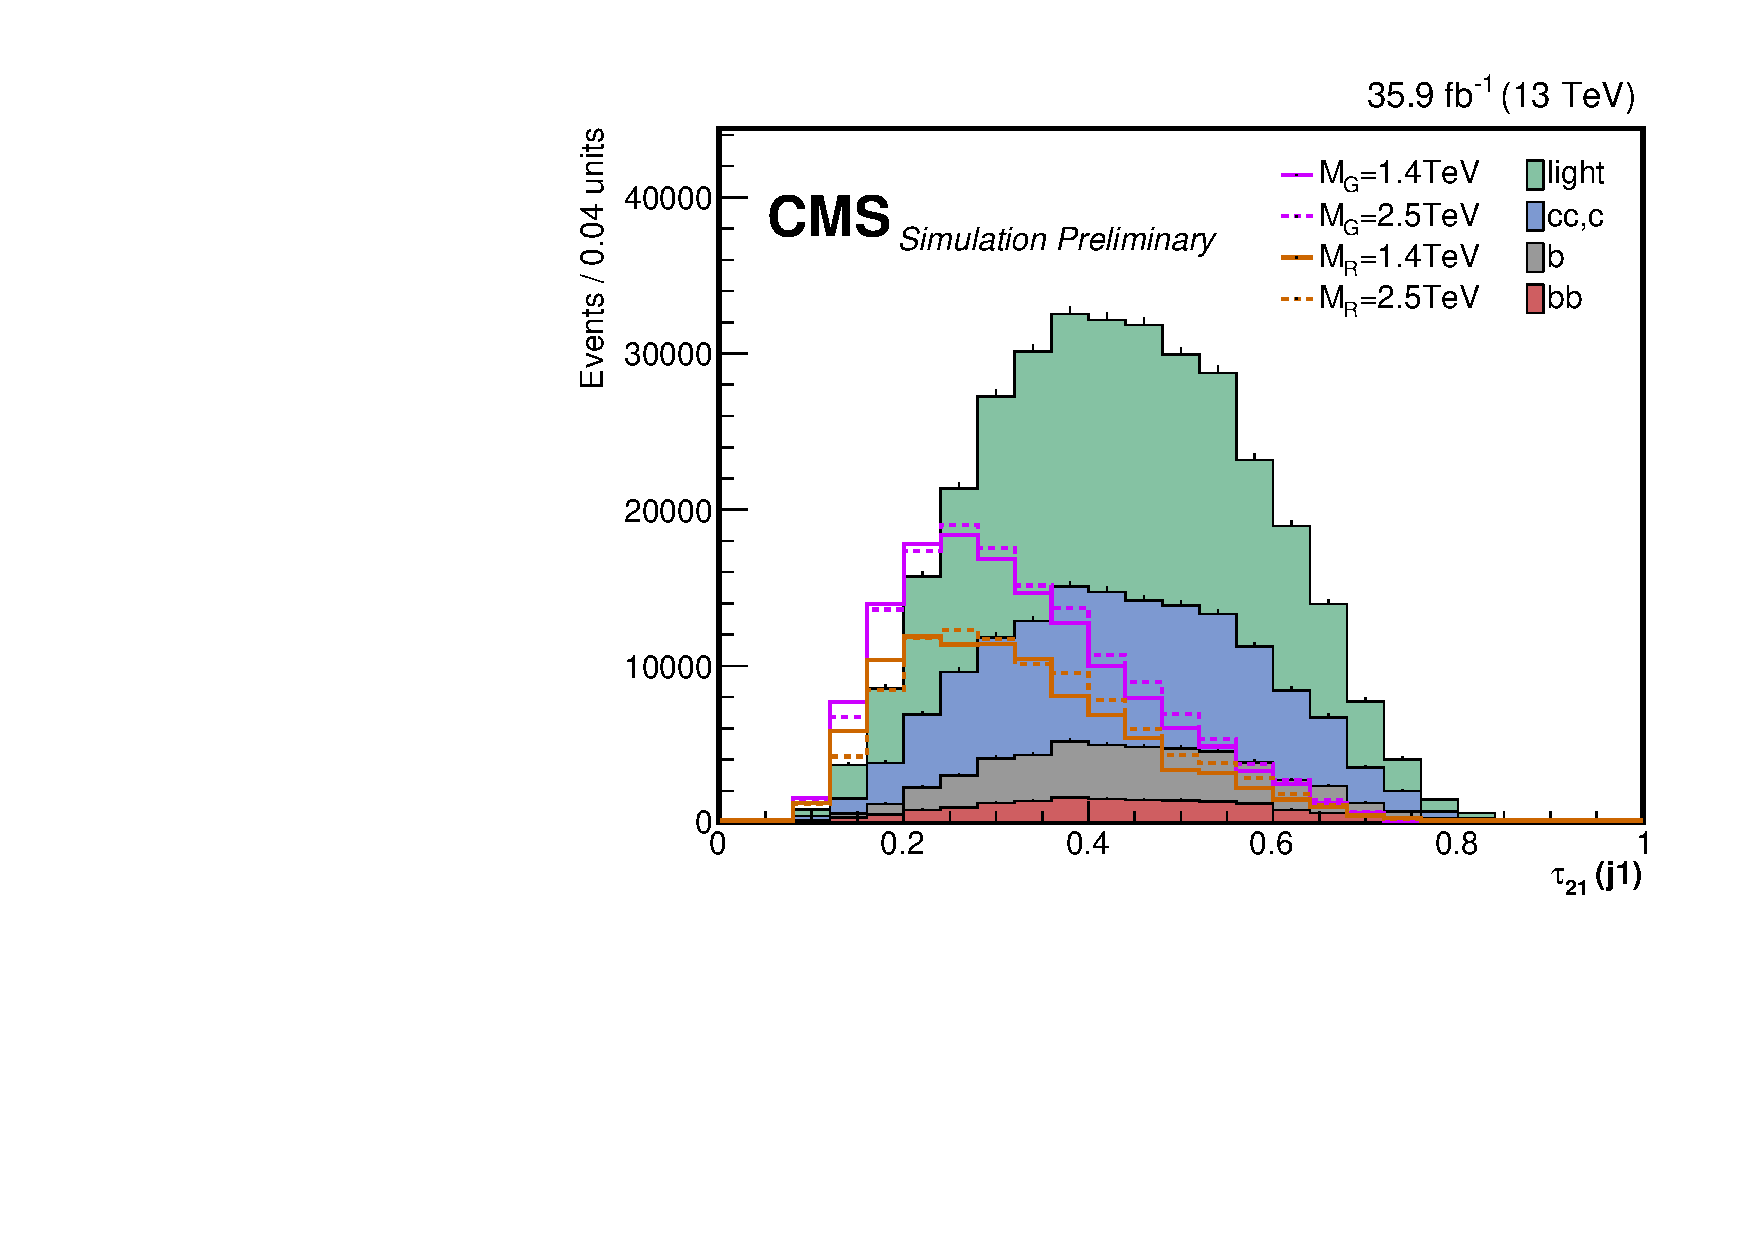
\includegraphics[width=0.5\textwidth]{Figures/MC_N1/puppiTau21_j0.pdf} &
%    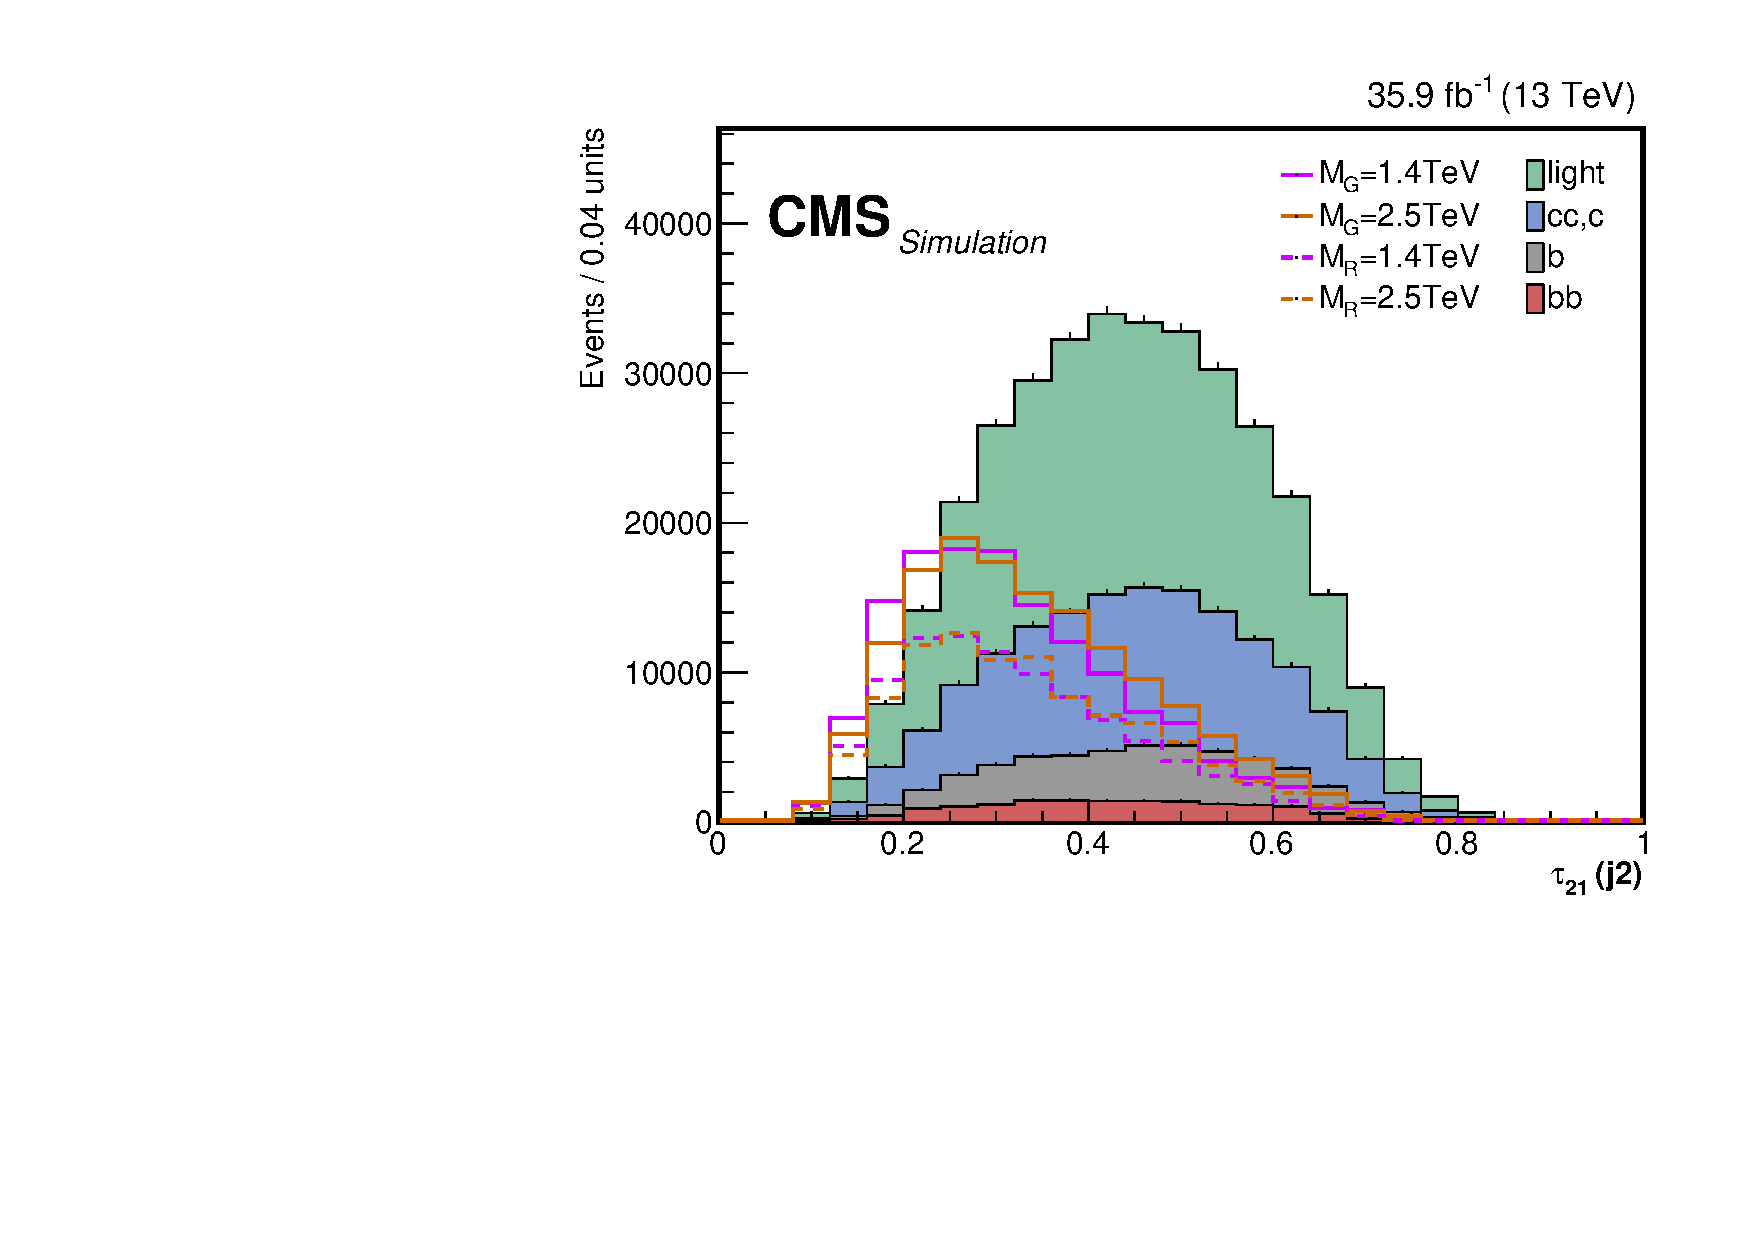
\includegraphics[width=0.5\textwidth]{Figures/MC_N1/puppiTau21_j1.pdf} \\
%     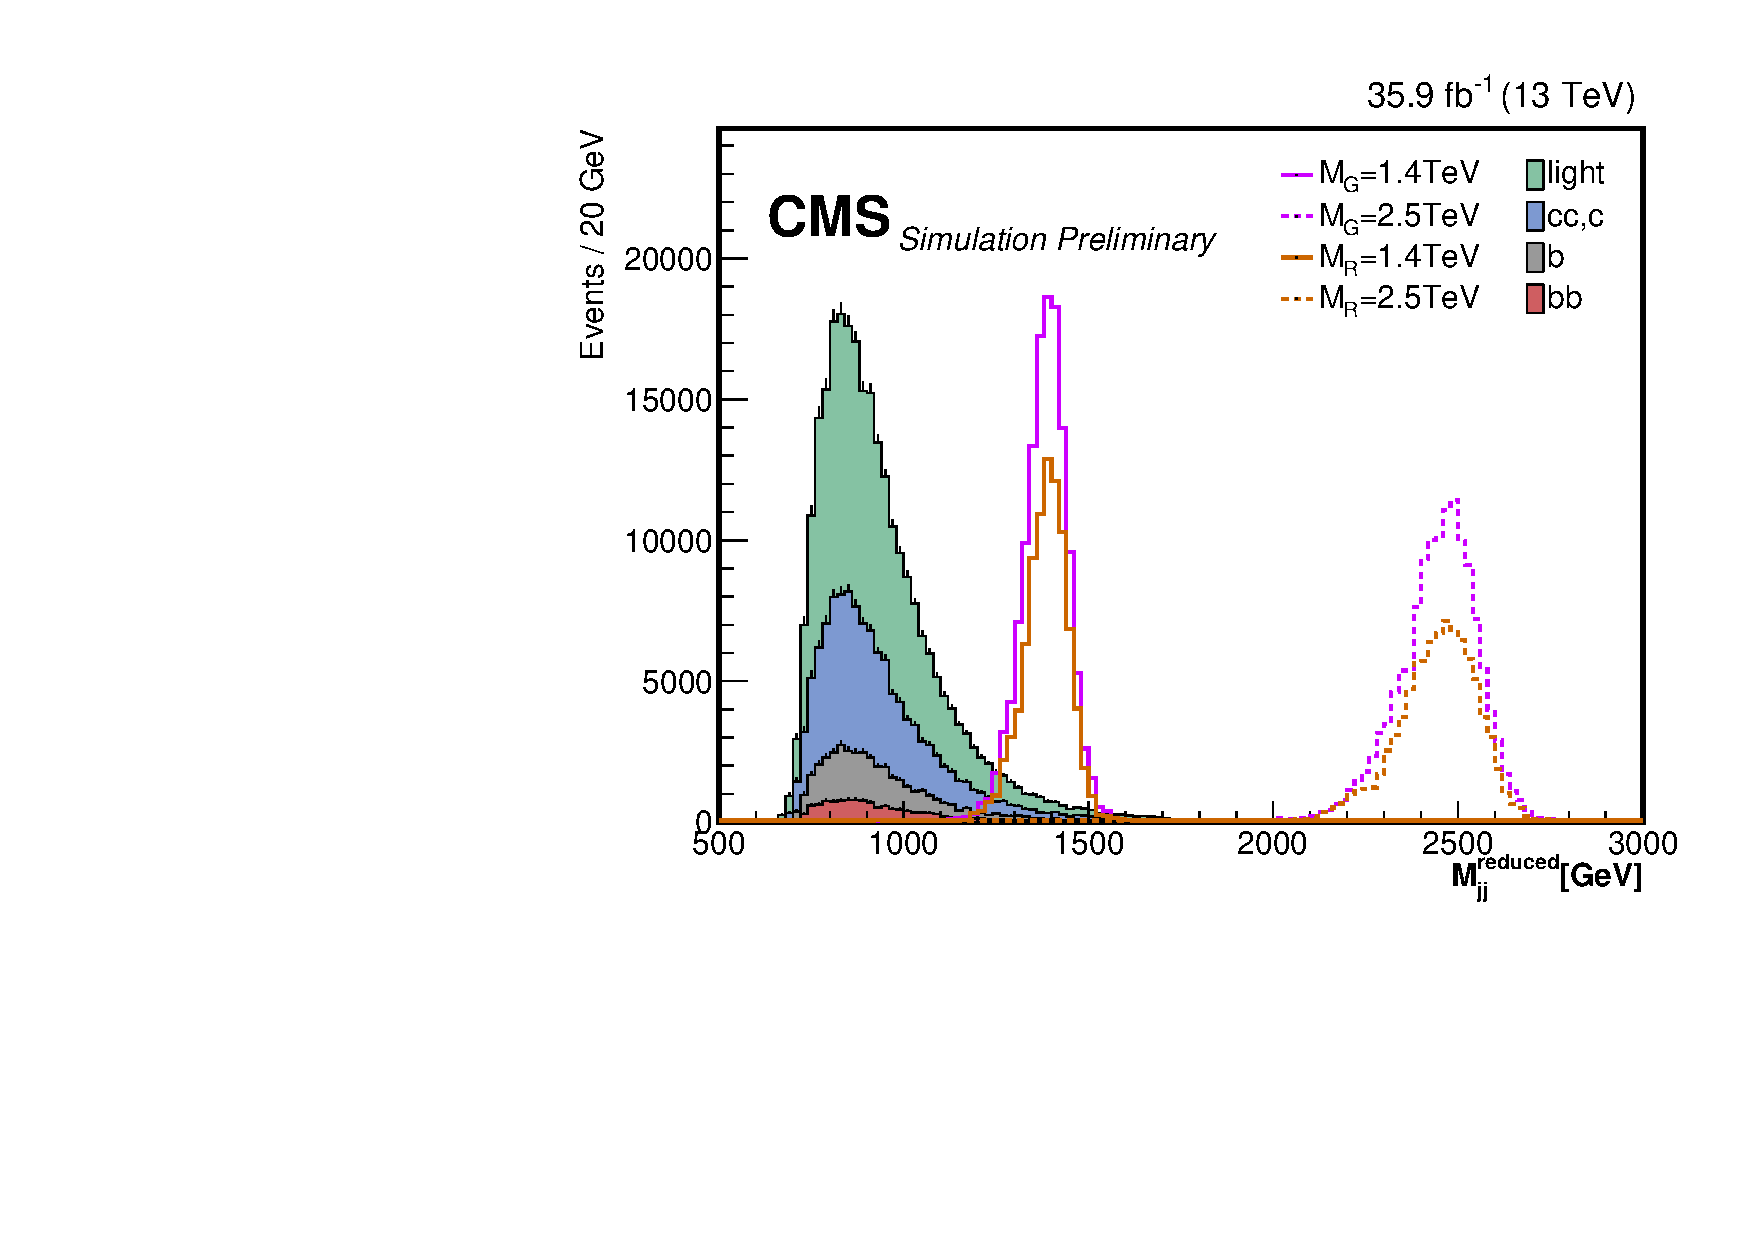
\includegraphics[width=0.5\textwidth]{Figures/MC_N1/totalMassRed.pdf} &
%    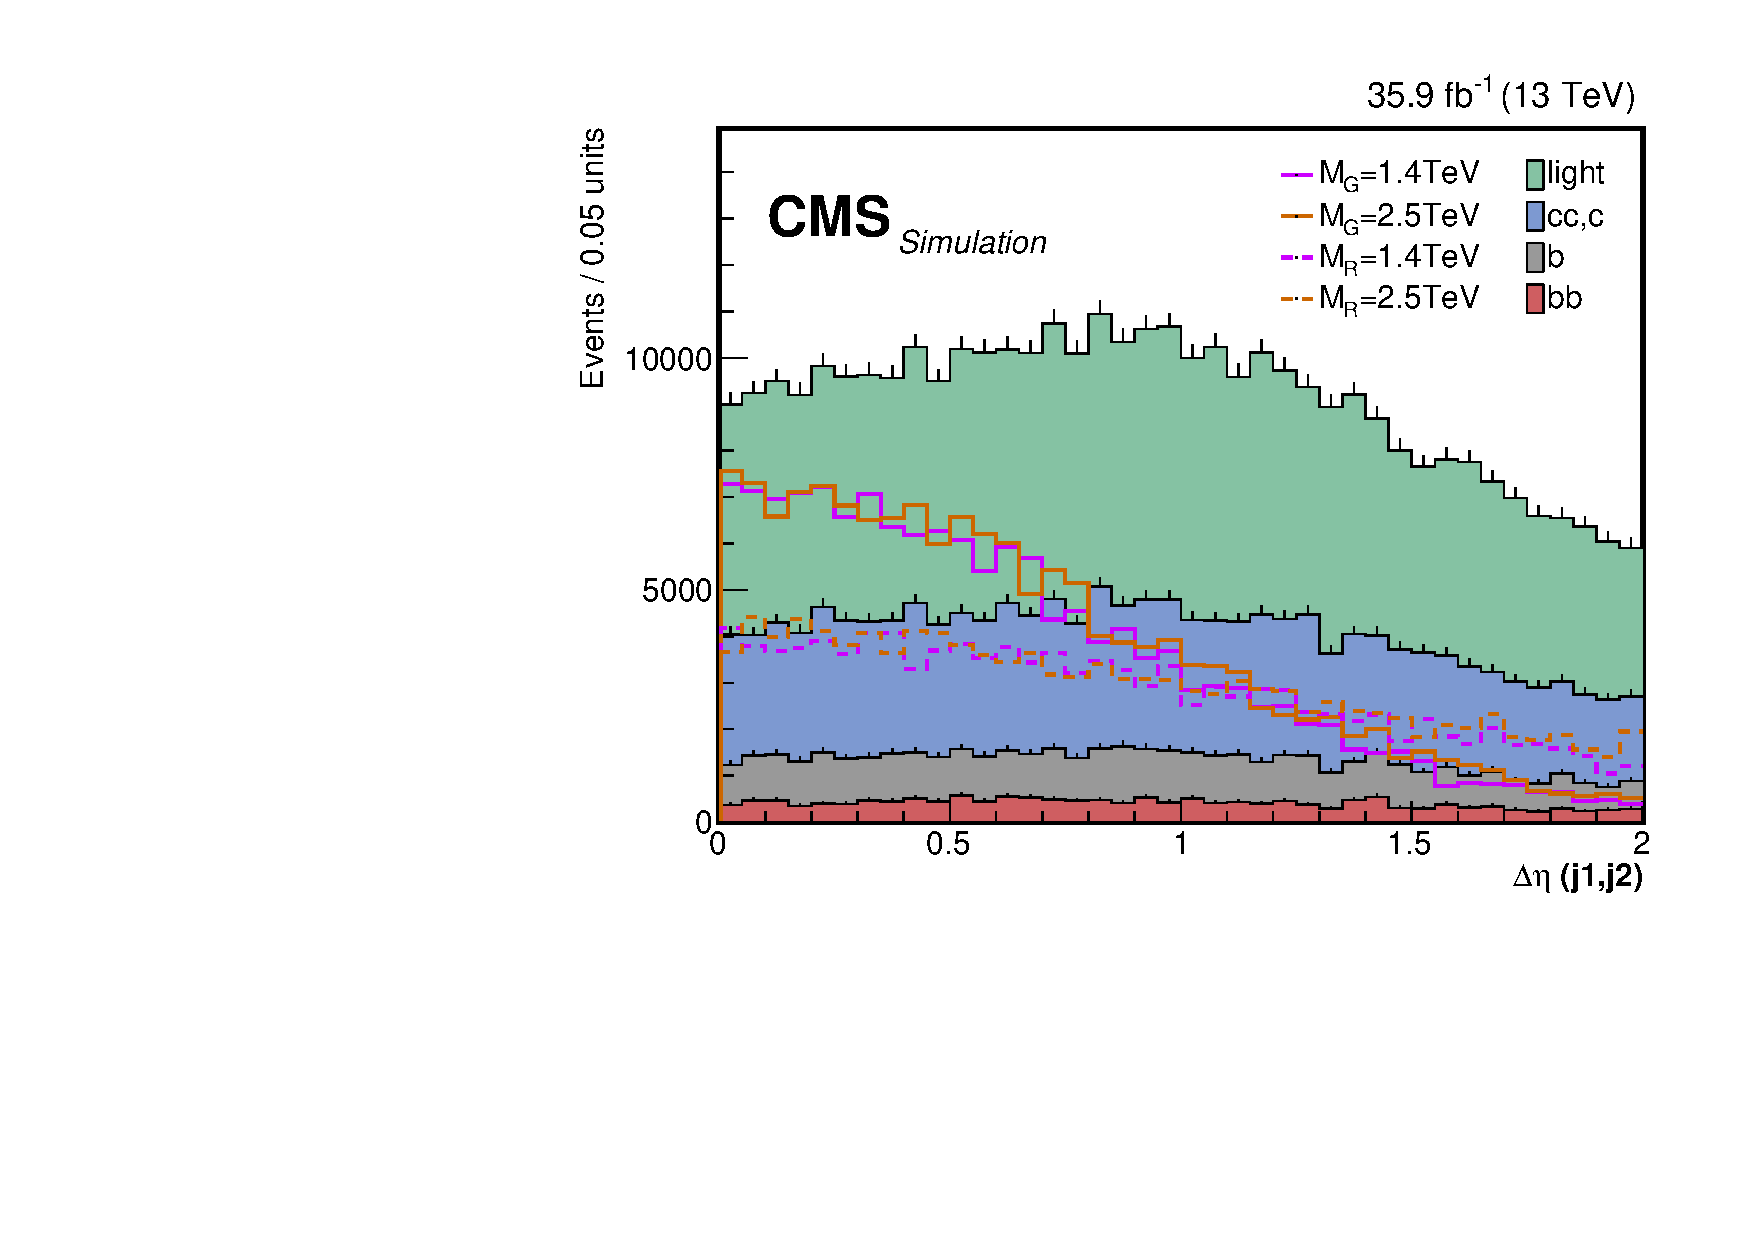
\includegraphics[width=0.5\textwidth]{Figures/MC_N1/deltaEta.pdf} \\
%  \end{tabular}
%  \caption{The comparison of signal and background. The signals of $M_{X}$ = 1.4 TeV and 2.5 TeV from both models are shown. The cross section is set to 20 pb in the figures. Multi-jet events are seperated into four categories summarized in the table 2.10. From top to buttom are the comparison of PUPPI soft-drop mass, $\tau _{21}$ of leading (left) and next leading (right) AK8 jet, the reduced mass (buttom left), and |$\Delta \eta $ (the two leading AK8 jets)| (buttom right).}
%  \label{fig:hvt_brs}
%\end{figure}